\documentclass{Resources/UoBLab1}
\pubyear{2018}
\subjectarea{Computational Vision}
\usepackage{listings}
\usepackage{hyperref}
\usepackage{amsmath}
\usepackage[english]{babel}
\usepackage{minted}
\usepackage{float}

% \usepackage[utf8]{inputenc}
\RecustomVerbatimEnvironment{Verbatim}{BVerbatim}{}

% \documentclass{article}
 



\begin{document}
\firstpage{1}

\title{Edge Detection}
\author{Charles de Freitas}
\course{Msc Computer Science}
\school{School of Computer Science}
\date{13th December 2018}
\keywords{Filtering, Smoothing}

\maketitle

\section{Laplacian of Gaussian}
Laplacian of Gaussian refers to convolution of a Gaussian smoothing mask with a Laplacian filter.
The Laplacian is a 2-D isotropic measure of the 2nd spatial derivative of an image.\cite{Laplacian}
A small sample Laplacian as as follows:
\[
\begin{bmatrix}
    0 & 1 & 0 \\
    1 & -4 & 1 \\
    0 & 1 & 0
\end{bmatrix}
\]
This is an example of a negative peek Laplacian, but inverting all the elements would work too. The change in sign across the Laplacian highlights rapid intensity change due to having such a sharp gradient across itself. Without smoothing, image noise will cause these rapid changes in intensity.
Since MATLAB includes a function for calculating the discrete Laplacian, we can simply perform
del2(img) on the image, then convolve this onto the Gaussian.
(This is because it requires less computations to convolve the two smaller matrices first than to apply them sequentially to the image.)
The final step is to refine the edges through zero crossing, this has been achieved by \textit{checking neighbours} of an element to change changes in sign.

\subsection{Laplacian of Gaussian}

\inputminted[fontsize=\scriptsize]{octave}{Resources/code/LoG.m}

\subsection{Zero Crossing}

\inputminted[fontsize=\scriptsize]{octave}{Resources/code/check_neighbours.m}\label{code:check_neighbours}

Changes in sign will represent an edge since the result of \textbf{LoG} is a differential image.

% \autoref{fig:shakey}
\begin{figure}
    \begin{center}
        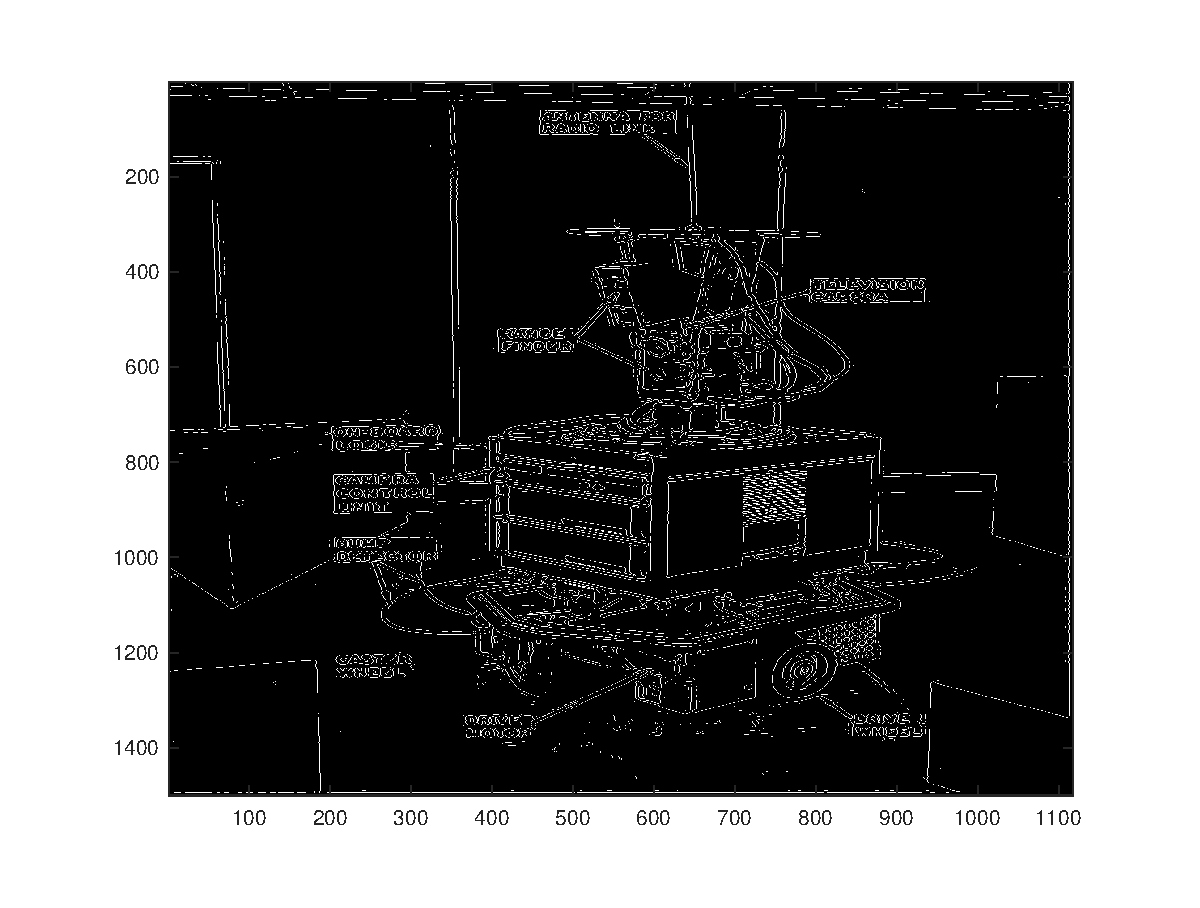
\includegraphics[scale=0.25]{Resources/images/LoG.eps}
        % \caption{Laplacian of Gaussian for a Gaussian of \[\bar{X} = 0 \sigma = 1\] and range 5}
        \label{fig:shakey}
    \end{center}
\end{figure}

The resulting image is Laplacian of Gaussian where the Gaussian is of \[\bar{x}=0,\sigma=2.5\]
This has produced a very clean image, if you wanted
% \clearpage




\section{Cell Detection}
\subsection{Filters}
\subsubsection{Sobel in X}
\[
\begin{bmatrix}
    -1 & 0 & 1 \\
    -2 & 0 & 2 \\
    -1 & 0 & 1
\end{bmatrix}
\]
\subsubsection{Sobel in Y}
\[
\begin{bmatrix}
    1 & 2 & 1\\
    0 & 0 & 0\\
    -1 & -2 & -1
\end{bmatrix}
\]
\subsubsection{Roberts in X}
\[
\begin{bmatrix}
    1 & 0\\
    0 & -1
\end{bmatrix}
\]
\subsubsection{Roberts in Y}
\[
\begin{bmatrix}
    0 & -1\\
    1 & 0
\end{bmatrix}
\]
\subsubsection{First Order Laplacian}
\[
\begin{bmatrix}
    0.1897 & 0.1741 & 0 & -0.1741 & -0.1897
\end{bmatrix}
\]
\clearpage
\textbf{ab\_max} applies the given filter to the image and returns the larges value in the resulting array. This is as to create an appropriate range of thresholds for the image. With this range of thresholds, an array of resultant images is produced.

\inputminted[fontsize=\scriptsize]{octave}{Resources/code/filterxy.m}

In the case of Roberts, the end function is:\\


\inputminted[fontsize=\scriptsize]{octave}{Resources/code/roberts.m}



Whereas for Laplacian you only need to convolve the single 2D matrix onto your smoothed image: 

\inputminted[fontsize=\scriptsize]{octave}{Resources/code/lap.m}

\subsection{Variable Smoothing}
\begin{enumerate}
	\item Create a set of Gaussian masks is produced for each filter.
	\item Create $\Omega$, a linear space bounded by 0 and the largest value possible for a given smoothed image.
	\item Apply the given smoothed filter for $\omega$ where $\omega \in \Omega$
	\item From the resulting set, calculate \textbf{TPR} and \textbf{FPR}.
	\item Repeate for all Gaussians and return a set of coortinates.
	\item Plot the set that contains the shortest distance to \((0,1)\)
	\item Repeate for all filters and respective Gaussians.
\end{enumerate}
\subsubsection*{Tuning}
Since each filter behaves differently, an appropriate set of Gaussian masks must be selected for each.
Starting with fixed values of \begin{math}
\bar{X} = 0 ,  \sigma{} = 1
\end{math}
and a range of
\lstinline[language=MATLAB]{0:1:10}\footnote[2]{From 0 to 10 and stepping by 1}.\\\autoref{fig:1to10}


\begin{figure}[h]
    \begin{center}
		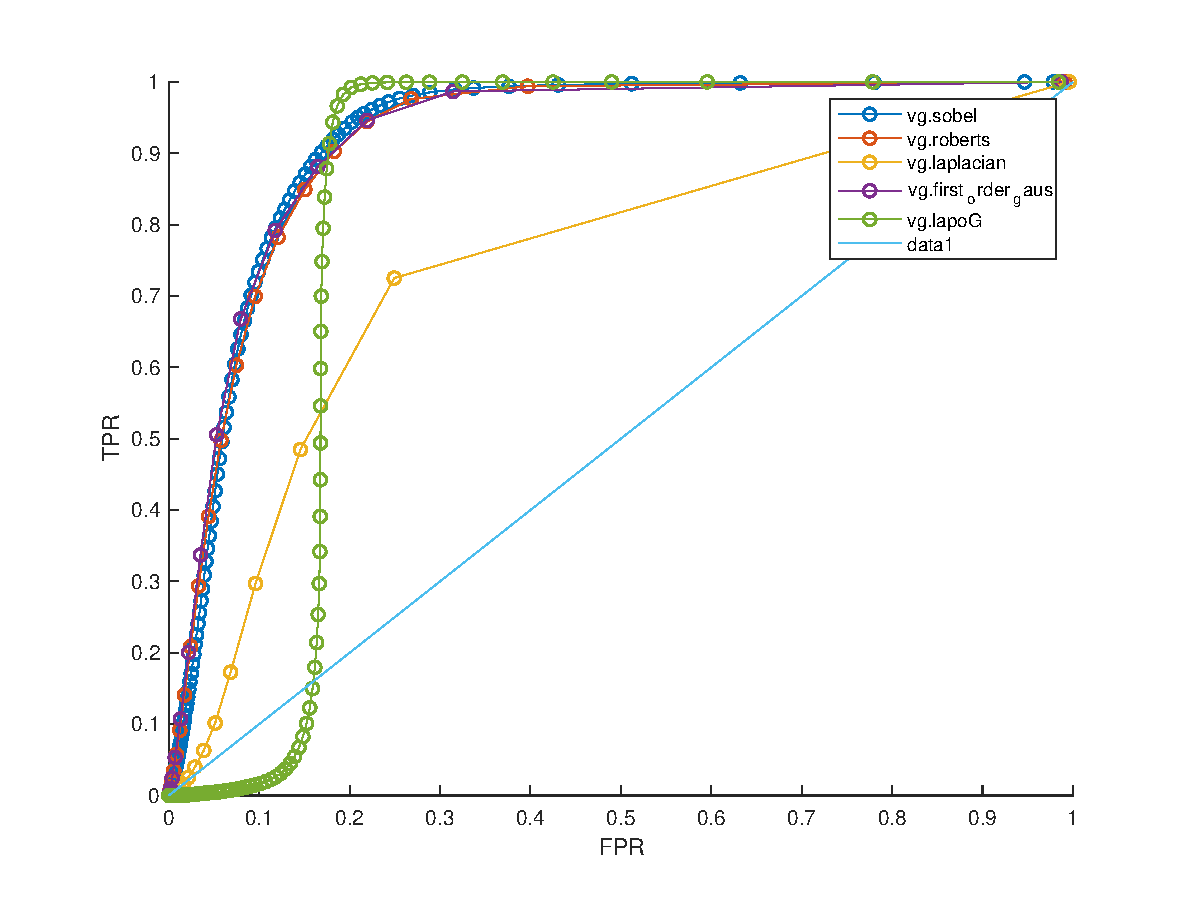
\includegraphics[scale=0.4]{Resources/images/all_dots.eps}
		\caption{Optimal curves when tested with identical Gaussians of size 0-10 on '9343 AM.bmp'}
        \label{fig:1to10}
    \end{center}
\end{figure}
\begin{figure}[h]
    \centering
    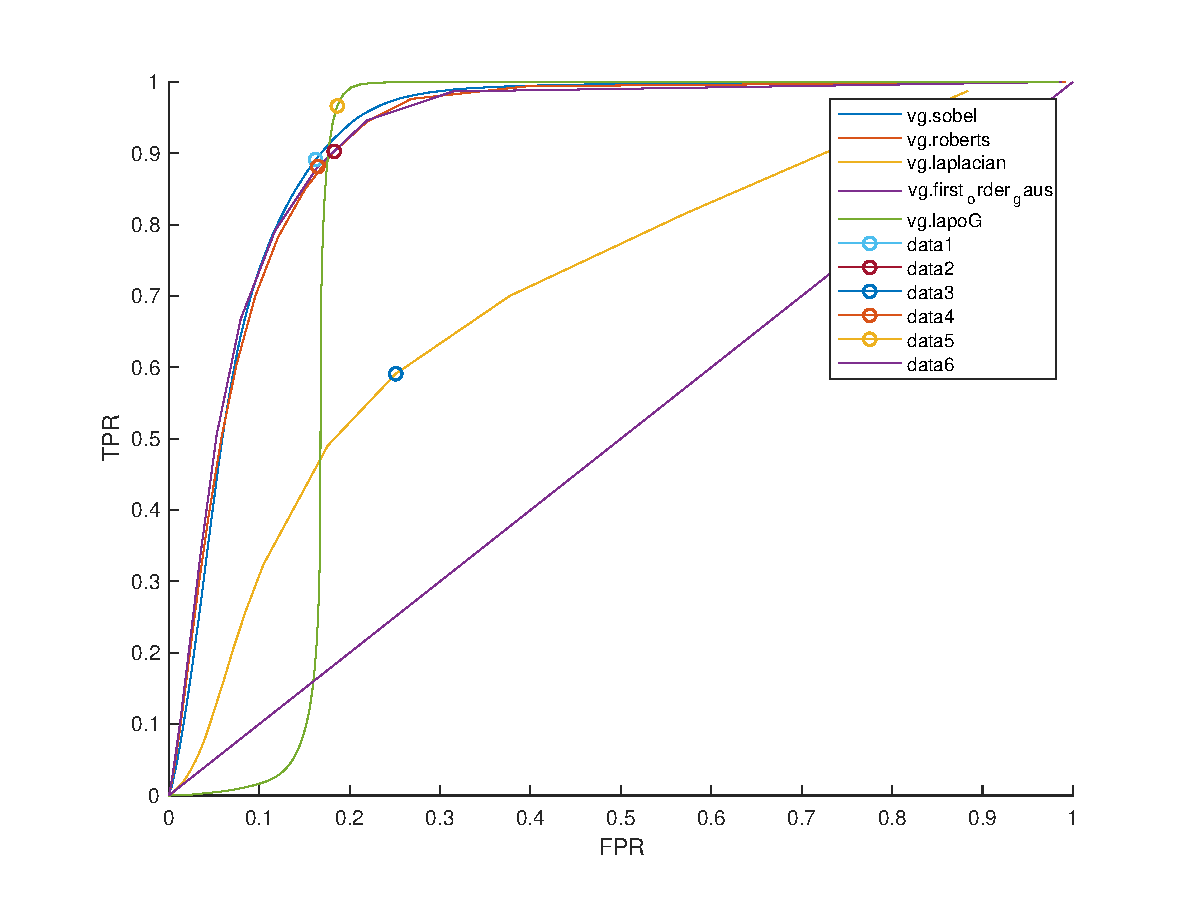
\includegraphics[scale=0.4]{Resources/images/best.eps}
    \caption{ROC space of each curve with most optimal value highlighted for '9343 AM.bmp'}
    \label{fig:best}
\end{figure}
\section{Results}
\begin{table}[h]
\begin{tabular}{llllll}
\hline
            & Sobel  & Roberts & Gaussian  & LoG    & Laplacian \\
      \hline
Specificity & 0.8376 & 0.817   & 0.8352    & 0.8164 & 0.7449    \\
Sensitivity & 0.8913 & 0.9027  & 0.8814    & 0.9464 & 0.5910    \\
\hline
\end{tabular}
\caption{Scores for '9343 AM.bmp}
\label{tab:img1}
\end{table}

\begin{table}[]
\begin{tabular}{llllll}
\hline
            & Sobel  & Roberts & Gaussian & LoG    & Laplacian \\ \hline
Specificity & 0.8514 & 0.8569  & 0.8363   & 0.8005 & 0.7204    \\
Sensitivity   & 0.8698 & 0.8525  & 0.8773   & 0.9353 & 0.5534    \\ \hline
\end{tabular}
\caption{Average of scores across all three images}
\label{tab:avr}
\end{table}
Sobel,  Roberts and First order Gaussian all give very similar results. This is due to them all being differential operators and in effect calculating edges through the same method, with varying degrees of success.\par
When smoothed with the same set of Gaussians, Laplacian Results in very few values past (0.1,0.1), this is because smoothing the image results in gradual changes of intensity. This is made more viable by applying much smaller Gaussians.

\section{Evaluation}
As you can see Laplacian over Gaussian, there is a very small change in threshold required to cause for almost perfect TPR, however due to the high clustering of data near the origin, it is worse than the randomly guessing in the vast majority of cases. 
Due to these properties, this would make it a highly effective filter for an image that has minimal noise, but will struggle otherwise.
The clustering of data can still be used if the point where it is no longer worse is calculated, the result can simply be inverted for these values.\par
The derivative filters on the other hand, while note having as high sensitivity, average a higher specificity, achieve a higher specificity; making them more effective in cases with more noise.\par
The Laplacian filter could be considered an adequate choice in both cases since it achieves mediocre scores in both respects, reducing the risk of false positives, but also that of true positives.

\begin{figure}[h]
    \centering
    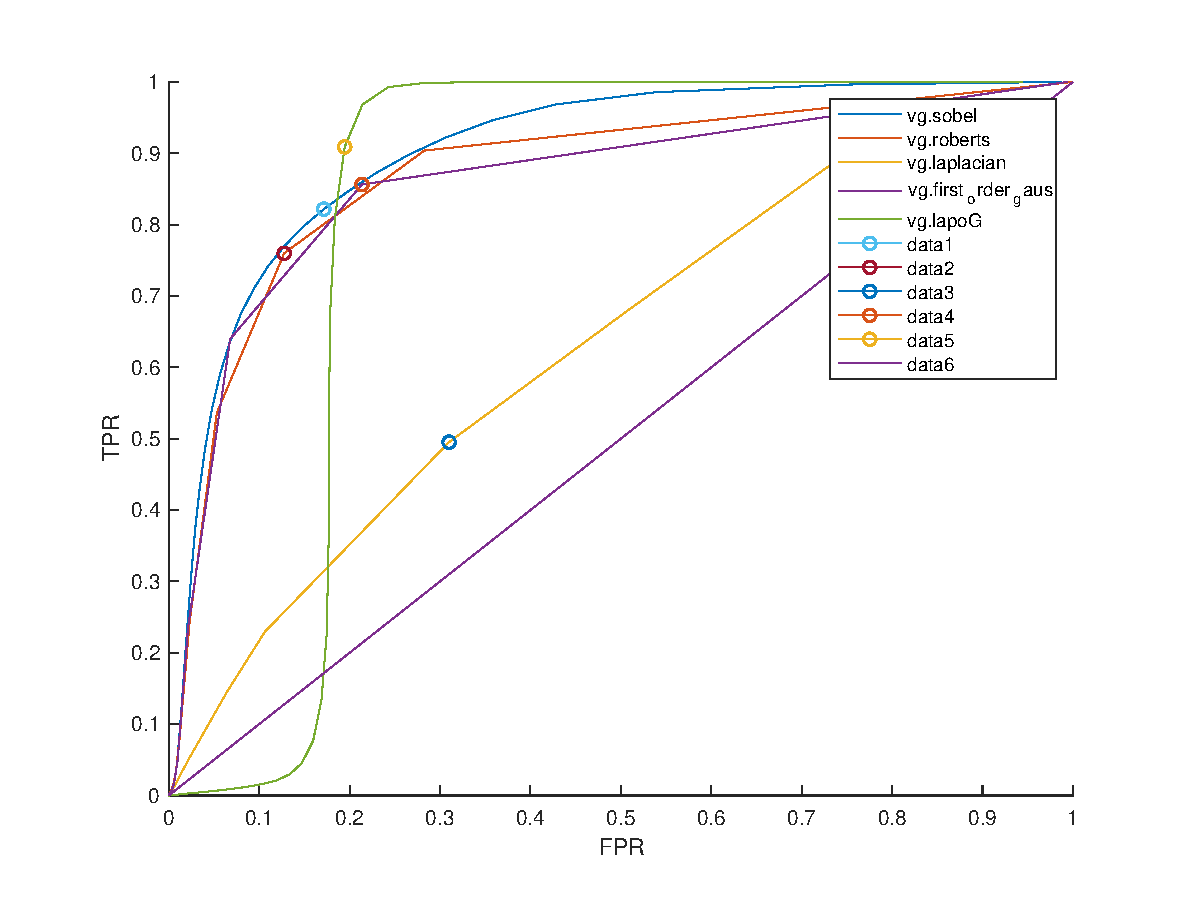
\includegraphics[scale=0.4]{Resources/images/best2.eps}
    \caption{Optimal curves when tested with identical Gaussians of size 0-10 on '43590 AM.bmp'}
    \label{fig:img2}
\end{figure}
\begin{figure}[h]
    \centering
    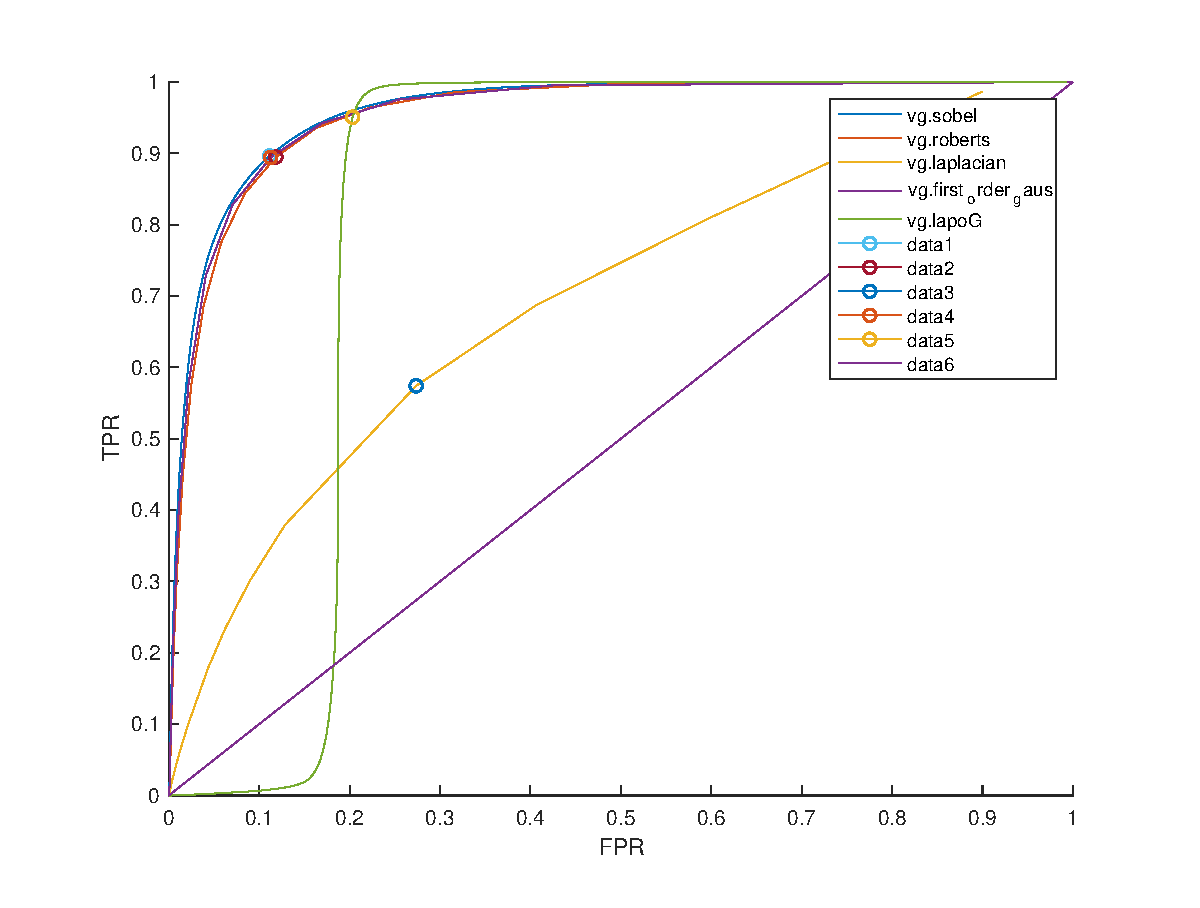
\includegraphics[scale=0.4]{Resources/images/best3.eps}
   \caption{Optimal curves when tested with identical Gaussians of size 0-10 on '10905 JL.bmp'}
    \label{fig:img3}
\end{figure}

\begin{thebibliography}{}

    \bibitem{Laplacian}
    \url{https://homepages.inf.ed.ac.uk/rbf/HIPR2/log.htm}
    \bibitem{del2}
    \url{https://uk.mathworks.com/help/matlab/ref/del2.html}
\end{thebibliography}

\end{document}
